%%
%% Copyright 2022 OXFORD UNIVERSITY PRESS
%%
%% This file is part of the 'oup-authoring-template Bundle'.
%% ---------------------------------------------
%%
%% It may be distributed under the conditions of the LaTeX Project Public
%% License, either version 1.2 of this license or (at your option) any
%% later version.  The latest version of this license is in
%%    http://www.latex-project.org/lppl.txt
%% and version 1.2 or later is part of all distributions of LaTeX
%% version 1999/12/01 or later.
%%
%% The list of all files belonging to the 'oup-authoring-template Bundle' is
%% given in the file `manifest.txt'.
%%
%% Template article for OXFORD UNIVERSITY PRESS's document class `oup-authoring-template'
%% with bibliographic references
%%

%%%CONTEMPORARY%%%
\documentclass[unnumsec,webpdf,contemporary,large]{oup-authoring-template}%
%\documentclass[unnumsec,webpdf,contemporary,large,namedate]{oup-authoring-template}% uncomment this line for author year citations and comment the above
%\documentclass[unnumsec,webpdf,contemporary,medium]{oup-authoring-template}
%\documentclass[unnumsec,webpdf,contemporary,small]{oup-authoring-template}

%%%MODERN%%%
%\documentclass[unnumsec,webpdf,modern,large]{oup-authoring-template}
%\documentclass[unnumsec,webpdf,modern,large,namedate]{oup-authoring-template}% uncomment this line for author year citations and comment the above
%\documentclass[unnumsec,webpdf,modern,medium]{oup-authoring-template}
%\documentclass[unnumsec,webpdf,modern,small]{oup-authoring-template}

%%%TRADITIONAL%%%
%\documentclass[unnumsec,webpdf,traditional,large]{oup-authoring-template}
%\documentclass[unnumsec,webpdf,traditional,large,namedate]{oup-authoring-template}% uncomment this line for author year citations and comment the above
%\documentclass[unnumsec,namedate,webpdf,traditional,medium]{oup-authoring-template}
%\documentclass[namedate,webpdf,traditional,small]{oup-authoring-template}

\onecolumn % for one column layouts

%\usepackage{showframe}

\graphicspath{{Fig/}}

% line numbers
%\usepackage[mathlines, switch]{lineno}
%\usepackage[right]{lineno}

\theoremstyle{thmstyleone}%
\newtheorem{theorem}{Theorem}%  meant for continuous numbers
%%\newtheorem{theorem}{Theorem}[section]% meant for sectionwise numbers
%% optional argument [theorem] produces theorem numbering sequence instead of independent numbers for Proposition
\newtheorem{proposition}[theorem]{Proposition}%
%%\newtheorem{proposition}{Proposition}% to get separate numbers for theorem and proposition etc.
\theoremstyle{thmstyletwo}%
\newtheorem{example}{Example}%
\newtheorem{remark}{Remark}%
\theoremstyle{thmstylethree}%
\newtheorem{definition}{Definition}


\newlength{\cslhangindent}
\setlength{\cslhangindent}{1.5em}
\newlength{\csllabelwidth}
\setlength{\csllabelwidth}{3em}
\newlength{\cslentryspacingunit} % times entry-spacing
\setlength{\cslentryspacingunit}{\parskip}
\newenvironment{CSLReferences}[2] % #1 hanging-ident, #2 entry spacing
 {% don't indent paragraphs
  \setlength{\parindent}{0pt}
  % turn on hanging indent if param 1 is 1
  \ifodd #1
  \let\oldpar\par
  \def\par{\hangindent=\cslhangindent\oldpar}
  \fi
  % set entry spacing
  \setlength{\parskip}{#2\cslentryspacingunit}
 }%
 {}
\usepackage{calc}
\newcommand{\CSLBlock}[1]{#1\hfill\break}
\newcommand{\CSLLeftMargin}[1]{\parbox[t]{\csllabelwidth}{#1}}
\newcommand{\CSLRightInline}[1]{\parbox[t]{\linewidth - \csllabelwidth}{#1}\break}
\newcommand{\CSLIndent}[1]{\hspace{\cslhangindent}#1}

\begin{document}

\journaltitle{Journal of the Royal Statistical Society, Series C (Applied Statistics)}
\DOI{DOI HERE}
\copyrightyear{2022}
\pubyear{2019}
\access{Advance Access Publication Date: Day Month Year}
\appnotes{Paper}

\firstpage{1}

%\subtitle{Subject Section}

\title[Impact of School Closures on COVID-19 by Age Cohorts]{Examining the Impact of School Closures on COVID-19 Infections in Europe and their Effects on Different Age Cohorts}

\author[1,$\ast$]{Damien Dupré\ORCID{0000-0001-8610-1045}}
\author[1]{Edgar Morgenroth\ORCID{0000-0002-9442-0561}}

\authormark{Dupré \& Morgenroth}

\address[1]{\orgdiv{Business School, Dublin City University}, \orgaddress{\street{Dublin}, \country{Ireland}}}

\corresp[$\ast$]{Corresponding author. \href{email:damien.dupre@dcu.ie}{damien.dupre@dcu.ie}}

\received{Date}{0}{Year}
\revised{Date}{0}{Year}
\accepted{Date}{0}{Year}

%\editor{Associate Editor: Name}

%\abstract{
%\textbf{Motivation:} .\\
%\textbf{Results:} .\\
%\textbf{Availability:} .\\
%\textbf{Contact:} \href{name@email.com}{name@email.com}\\
%\textbf{Supplementary information:} Supplementary data are available at \textit{Journal Name}
%online.}

\abstract{This paper provides a thorough analysis of COVID-19 case trends in selected European countries, focusing on the influence of different age groups. It explores the relationship between population size and confirmed case numbers, suggesting that larger countries tend to have higher case figures. The study investigates how various waves of the pandemic affect different age demographics, with older age groups being most affected by the initial wave and younger age groups more impacted by subsequent waves.
Using a Generalised Additive Model (GAM), the research assesses the impact of school closures on COVID-19 cases, revealing a decreasing non-linear effect across all countries examined. Following school closures, distinct trends emerge among age groups: ages 0 to 4 experience a decrease, ages 5 to 14 see an increase, and ages 15 to 24 initially surge then decline. Transfer Entropy calculations uncover imbalances in age group influences, with certain age groups predicting changes in others.
Consistent patterns across countries are identified, such as younger cohorts influencing older cohorts in Austria, Germany, and the Netherlands, while Portugal and Spain show the opposite trend. These findings deepen our understanding of COVID-19 dynamics in Europe, providing valuable insights for targeted public health strategies and interventions.}
\keywords{COVID-19, School Closures, Causality, Generalised Additive Model, Transfer Entropy}

% \boxedtext{
% \begin{itemize}
% \item Key boxed text here.
% \item Key boxed text here.
% \item Key boxed text here.
% \end{itemize}}

\maketitle








\hypertarget{introduction}{%
\section{Introduction}\label{introduction}}

A wide range of non-pharmaceutical interventions (NPI) were enacted to control the spread of COVID-19, especially before the availability of effective vaccines. Due to their social mixing patterns, children have been identified as an age group that can drive the spread of respiratory infections such as influenza (Moser and White, 2018), and school closures were found to be effective in mitigating the spread of influenza H1N1 in Japan in 2009 (Kawano and Kakehashi, 2015). It is therefore not surprising that school closures were one of the NPIs that were introduced in many countries to stop the spread of COVID-19. They were used particularly during the initial wave of the pandemic and during subsequent waves when case numbers were high.

Recently, a body of literature has shown various negative consequences on child development and health due to school closures. School closures have been found to have negatively affected child mental health (Moulin et al., 2022), nutrition/obesity (Sugimoto et al., 2023), and education (Lerkkanen et al., 2023). Some governments are now questioning their decisions to close schools (De Simone and Mourao, 2021). For example, the German health minister Karl Lauterbach, in an interview with one of Germany's publicly funded television stations, admitted that ``in retrospect it had been wrong to keep schools and childcare closed for so long'' ({``ARD tagesschau,''} 2023).

Even if school closures had negative consequences for children, they might nevertheless have been effective at stopping the spread of COVID-19. However, analysis on the effectiveness of school closures on the spread of COVID-19 remains inconclusive. Alfano (2022) in a study of a panel of European countries found that school closures were associated with a reduced COVID-19 incidence. In contrast, Walsh et al. (2021) in a review of 40 studies covering 150 countries concluded that the effectiveness of school closures was uncertain, with 60\% having identified no impact and pointing to the potential for the analysis to be affected by confounding factors and collinearity. The latter shortcomings suggest that it is hard to draw firm inferences, as even a positive result may not imply causality.

This paper investigates the dynamics of COVID-19 across age groups and how this was affected by school closures. This allows us to identify the effect of school closure on the evolution of COVID-19 cases in other age groups and particularly on older and more vulnerable age groups, including parents, grandparents, and relatives about which little is known.

We identify the relationship between the school closures and case numbers in different age groups using Generalized Additive Models (GAM), which are more flexible than conventional Vector Autoregressions, given that they allow for non-linear relationships between variables. Furthermore, compared to other methods such as Vector Autoregression, GAM can handle fixed and random smooth effects without making strict assumptions about linearity. Then, using the transfer entropy method, we evaluate the impact of case number changes between age groups in order to identify if school closure has secondary repercussions in the household. Transfer entropy can adapt to changes in the underlying system dynamics over time. It does not assume stationarity and can capture evolving causal relationships, making it suitable for studying dynamic systems and non-stationary processes such as COVID-19 contaminations.

\hypertarget{influence-of-school-closure}{%
\subsection{Influence of School Closure}\label{influence-of-school-closure}}

Once it was clear that COVID-19 spreads from person to person, it was natural that governments were advised to enact measures to reduce social contact in order to reduce the spread of the virus. Therefore, it is legitimate to believe that by closing schools, a reduction of the contaminations would be observed in the younger age groups. However, the efficiency of school closure on the reduction of COVID-19 cases is still questioned (Bayham and Fenichel, 2020; Esposito et al., 2021). While some research has found that school closures contribute to limit or to reduce the growth rate of confirmed cases after implementation (Stage et al., 2021; Sugishita, 2020), others did not observe a change in the evolution of COVID-19 cases (Chang et al., 2020; Iwata et al., 2020). For instance, a controlled comparison between similar localities in Japan with schools closed and schools open did not reveal any evidence that school closures reduced the spread of COVID-19 (Fukumoto et al., 2021). If the school closure had a real impact on the evolution of confirmed COVID-19 cases, it should be possible to observe a decrease or at least an inflection in the trend of its evolution among younger age groups.

\hypertarget{causal-relationship-between-age-groups}{%
\subsection{Causal Relationship Between Age Groups}\label{causal-relationship-between-age-groups}}

A second implicit belief regarding the effect of school closure on the spread of COVID-19 is that school not only influences the spread of the virus among children and teenagers but also has a knock-on effect on the spread of the virus in older age groups, also called Secondary Attack Rate (SAR). The contaminated children and teenagers would bring the virus back home and would pass the virus on to their parents and relatives. For example, research investigating the contamination in the household network not only revealed an exceptionally high rate of secondary contamination but also that this contamination happened when the schools were closed (Soriano-Arandes et al., 2021).

Despite being reported in several clinical and epidemiological studies (Siebach et al., 2021; Zhen-Dong et al., 2020), multiple research have shown that the SAR from children to household members was lower than expected (Heavey et al., 2020; Hoek et al., 2020; Kim et al., 2021; Ludvigsson, 2020). However, the SAR of children and teenagers to the household member is likely to be age-dependent, with differences between infants, primary and secondary school children, and college students (Gras-Le Guen et al., 2021). If a secondary transmission from children and teenagers to household member has a significant influence, then a temporal causality relationship between their evolution should be observed.

To evaluate the impact of school closure on COVID-19 cases across different age groups, we first performed a non-linear time series regression to analyze the relationship between school closures and the number of COVID-19 cases in various age groups. In a second analysis, the transfer entropy method is employed to assess the influence of changes in case numbers between age groups, aiming to determine if school closures have secondary effects within households.

\hypertarget{estimation-methodology}{%
\section{Estimation Methodology}\label{estimation-methodology}}

\hypertarget{generalized-additive-model}{%
\subsection{Generalized Additive Model}\label{generalized-additive-model}}

The effect of school closure on the trend of daily COVID-19 cases is analyzed using a Generalized Additive Model (GAM). GAM is a flexible modeling approach that estimates non-linear relationships between variables. Compared to other methods such as Vector Autoregression, GAM can handle fixed and random smooth effects without making strict assumptions about linearity.

The GAM is fitted on the daily COVID-19 cases to test the hypothesis of a significant non-linear evolution of cases among age groups from 0 to 4, from 5 to 9, from 10 to 14, from 15 to 19, and from 20 to 24 (Wood, 2017). The model also estimates the overall non-linear effect by country, taking into account the interaction between age groups and countries as random intercepts and the interaction between time, countries, and the period of closure as random effects (Eq 1).

By estimating the degree of smoothness of a Bayesian spline smoothing using restricted fast maximum likelihood estimation (Wood, 2011), GAM identifies dynamic patterns underlying the evolution of COVID-19 cases reported while including the random effect of different age groups and countries as follows:

\begin{align*}
  \tag{1}
  n\prime_t &\sim Poisson(\mu_t) \\
  \log(\mu_t) &= \beta_0 + \beta_1\,wave_t + \beta_2\,country_t + \beta_3\,age\,group_t + \\
              & f_1(closure_t) + f_2(closure_t,country_t) + f_3(closure_t,age\,group_t)
\end{align*}

\noindent where \(n\prime_t\) represents the confirmed COVID-19 cases, assuming a Poisson distribution for the fitting (Loader, 2006), and \(t\) is the date corresponding to the confirmed COVID-19 cases. The response variable includes a specific random effect taking into account variation within waves of school closure, countries, and age groups. The terms \(f_1\) to \(f_3\) are smooth functions of the time since closure, the time since closure for each country, and the time since closure for each age group. The restricted maximum likelihood (REML) was used to avoid overfitting while estimating smoothing parameters. In order to accurately account for the autocorrelation arising from the time series data, the residuals are modeled using an AR1 error model. By incorporating the autoregressive component, the AR1 model acknowledges the dependence of each residual on its previous value, thus providing a comprehensive representation of the data's temporal dynamics.

\hypertarget{transfer-entropy}{%
\subsection{Transfer Entropy}\label{transfer-entropy}}

Transfer entropy (\(T\)) can be used to infer the temporal relationship between two time series \(X\) and \(Y\). This measure indicates whether changes in COVID-19 cases within a certain age group \(X\) can be used to reduce the uncertainty on the future COVID-19 cases within another age group \(Y\). If it does, \(T\) is considered evidence of a causal effect from the age group \(X\) to the age group \(Y\) (Schreiber, 2000). As such, Granger causality is a special case of transfer entropy applied to time series that are jointly Gaussian distributed (Barnett et al., 2009). Therefore, transfer entropy is a more robust analysis of time series, especially when applied to the impact of age cohorts on pandemic transmission (Kissler et al., 2020).

The influence of the evolution in COVID-19 cases across all age groups is evaluated using Shannon's transfer entropy, given by:

\begin{align}
  \tag{2}
  T_{ag\,x \rightarrow\,ag\,y}(k,l) = \sum_{ag\,x,ag\,y} p\left(ag\,x_{t+1}, ag\,x_t^{(k)}, ag\,y_t^{(l)}\right) \log \left(\frac{p\left(ag\,x_{t+1}| ag\,x_t^{(k)}, ag\,y_t^{(l)}\right)}{p\left(ag\,x_{t+1}|ag\,x_t^{(k)}\right)}\right)
\end{align}

\noindent where \(T_{ag\,x \rightarrow\,ag\,y}\) consequently measures the influence of the change dynamic from an age group \(X\) (or \(ag\,x\)) to another age group \(Y\) (or \(ag\,y\)) for every country (Eq 2).

The day-by-day difference in COVID-19 confirmed cases \(n\prime\prime_t\) is used to satisfy the stationary requirement for the calculation of Shannon's Transfer Entropy (Behrendt et al., 2019; Shannon, 1948).

\hypertarget{data}{%
\section{Data}\label{data}}

\hypertarget{covid-19-cases-per-age-group}{%
\subsection{COVID-19 cases per age group}\label{covid-19-cases-per-age-group}}

For the analysis, data on COVID case counts by age group are required. The number of COVID-19 cases per age group has been taken from the COVerAGE-DB project (Riffe et al., 2021). The COVerAGE-DB project consists of 3 data files: an ``Input'' data file that collects the official COVID-19 cases from 117 countries, the ``Output\_5'' data file, which is a projection of COVID-19 cases by a group of 5 years, and the ``Output\_10'' data file, which is a projection of COVID-19 cases by a group of 10 years. For our analyses, we have used the ``Output\_5,'' which deals with the heterogeneity of countries' reporting formats by using spline approximations when the data for this age bracket is not available for a country. Therefore, it allows a precise analysis between age groups under 24, while age groups of 25 and above are reduced to 10-year brackets, and groups above 64 are concatenated all together.

In order to cross-validate the data obtained after spline approximations, a comparison with the data published by the {``World health organization COVID-19 data''} (2022) reveals perfect similarities. The original data consist of 14,089,320 observations of 10 variables (117 distinct countries, region within the country, a unique observation code, the date of the observation, the gender, which can be male, female, or both, the age bracket by 5 years from 0 to 100, a confirmation of the age interval for each bracket, the total number of cases so far, the total number of deaths, and the total number of tests performed) from February 16, 2020 to January 20, 2022. After removing countries with missing and inconsistent values, only 22 are suitable for data analyses. However, to focus this analysis on geographically and culturally comparable countries, only 12 European countries are kept: Austria, Belgium, Bulgaria, Croatia, Estonia, France, Germany, Greece, Netherlands, Portugal, Slovakia, and Spain. The observations are reported in terms of the total number of COVID-19 cases per day from the start of the pandemic. The daily number of cases at a specific date \(n\prime_{t}\) is calculated with the difference between the total cases at a date \(t\) and the total cases at a date \(t-1\) (i.e., derivative 1). In addition, the change in the daily number of cases \(n\prime\prime_{t}\) between \(n\prime_{t}\) and \(n\prime_{t-1}\) has also been calculated (i.e., derivative 2).

\hypertarget{school-closure}{%
\subsection{School closure}\label{school-closure}}

To identify the impact of school closures on the number of cases, information regarding the school closures on a day-by-day basis is required, and this is taken from the ``UNESCO global education coalition'' (2022). For each day, in each country, the status of the schools is indicated as fully open, partially open, closed due to COVID-19, or closed due to an academic break. Because it would be difficult to measure the effect of school closures at a country level when schools are partially closed, only closures due to COVID-19 or due to an academic break are considered. Indeed, both are considered as closure at a country-wide level. Note that periods of closure longer than 21 days are compared for 28 days, regardless of whether the schools opened or not after 21 days. Any COVID-19 case numbers beyond the 28-day period are not relevant for evaluating the impact of school closures.

\hypertarget{results}{%
\section{Results}\label{results}}

The data show that the trend of confirmed COVID-19 cases follows similar patterns across the selected European countries, with scales following the size of the population in these countries (Figure \ref{fig:overall}). Thus, the bigger the country, the higher the total number of COVID-19 cases.

\begin{figure}
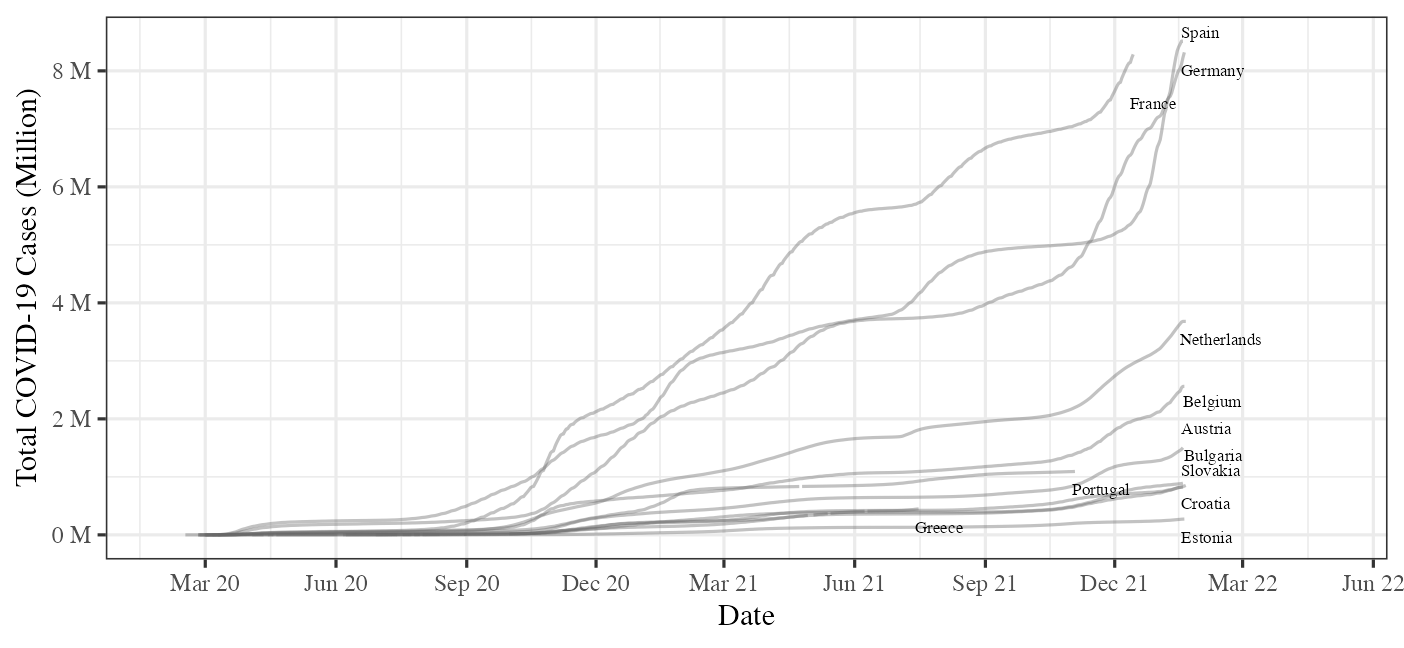
\includegraphics[width=\textwidth]{manuscript_files/figure-latex/overall-1} \caption{Cumulative COVID-19 cases number for selected European countries since the beginning of the pandemic. Source: COVerAGE-DB (Riffe et al., 2021).}\label{fig:overall}
\end{figure}

The evolution of COVID-19 cases reveals some similarities across all age groups. However, the influence of each wave on individual age groups also has some particularities (Figure \ref{fig:descriptive}). For example, the first wave was more important among the oldest age groups, whereas the third wave was more important among the youngest age groups.

\begin{figure}
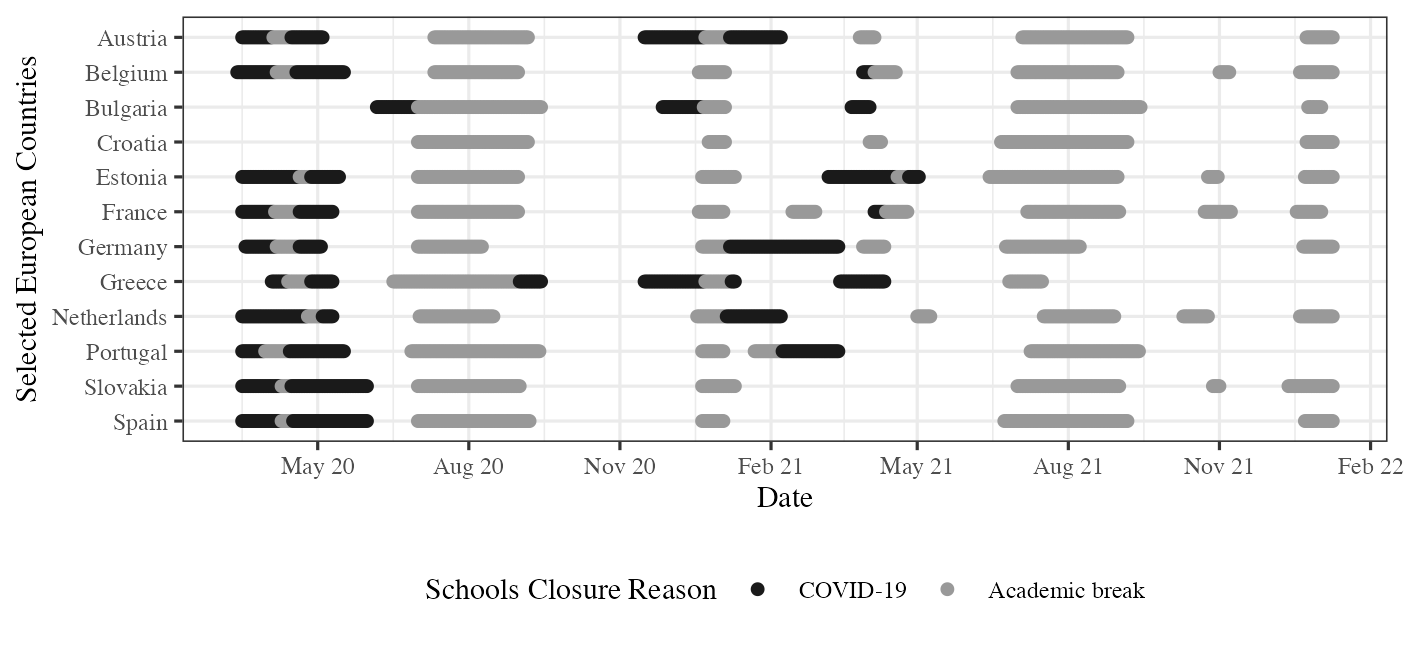
\includegraphics[width=\textwidth]{manuscript_files/figure-latex/descriptive-1} \caption{Periods of school closure since the beginning of the COVID-19 pandemic for selected European countries and their reason: regular academic break vs.~closure due to government decisions. Source: {``{UNESCO} global education coalition''} (2022).}\label{fig:descriptive}
\end{figure}

As outlined above, to evaluate the shape of the trend in the numbers of COVID-19 cases reported after the three school closures longer than 21 consecutive days, a GAM was fitted as described above, taking into account the overall effect across all the selected European countries, as well as the effect for age groups: 0 to 4, 5 to 9, 10 to 14, 15 to 19, and 20 to 24 years old. The obtained results satisfy the requirements to fit this model, which explains 77.2\% of the variation in COVID-19 cases.

Overall, the results revealed a decreasing non-linear effect of school closure at a country level for the selected European countries (Austria: \(\chi^2(5.75) = 2934.05\), \(p < 0.001\); Belgium: \(\chi^2(5.99) = 9805.66\), \(p < 0.001\); Bulgaria: \(\chi^2(5.92) = 158.24\), \(p < 0.001\); Croatia: \(\chi^2(5.45) = 681.91\), \(p < 0.001\); Estonia: \(\chi^2(5.9) = 1827.73\), \(p < 0.001\); France: \(\chi^2(5.96) = 6713.39\), \(p < 0.001\); Germany (\(\chi^2(5.97) = 4176.3\), \(p < 0.001\)); Greece: \(\chi^2(5.91) = 1306.4\), \(p < 0.001\); The Netherlands: \(\chi^2(5.97) = 14370.95\), \(p < 0.001\); Portugal: \(\chi^2(5.86) = 2423.35\), \(p < 0.001\); Slovakia (\(\chi^2(5.97) = 6628.69\), \(p < 0.001\); Spain: \(\chi^2(5.94) = 562.49\), \(p < 0.001\), see Figure \ref{fig:age}).

\begin{figure}
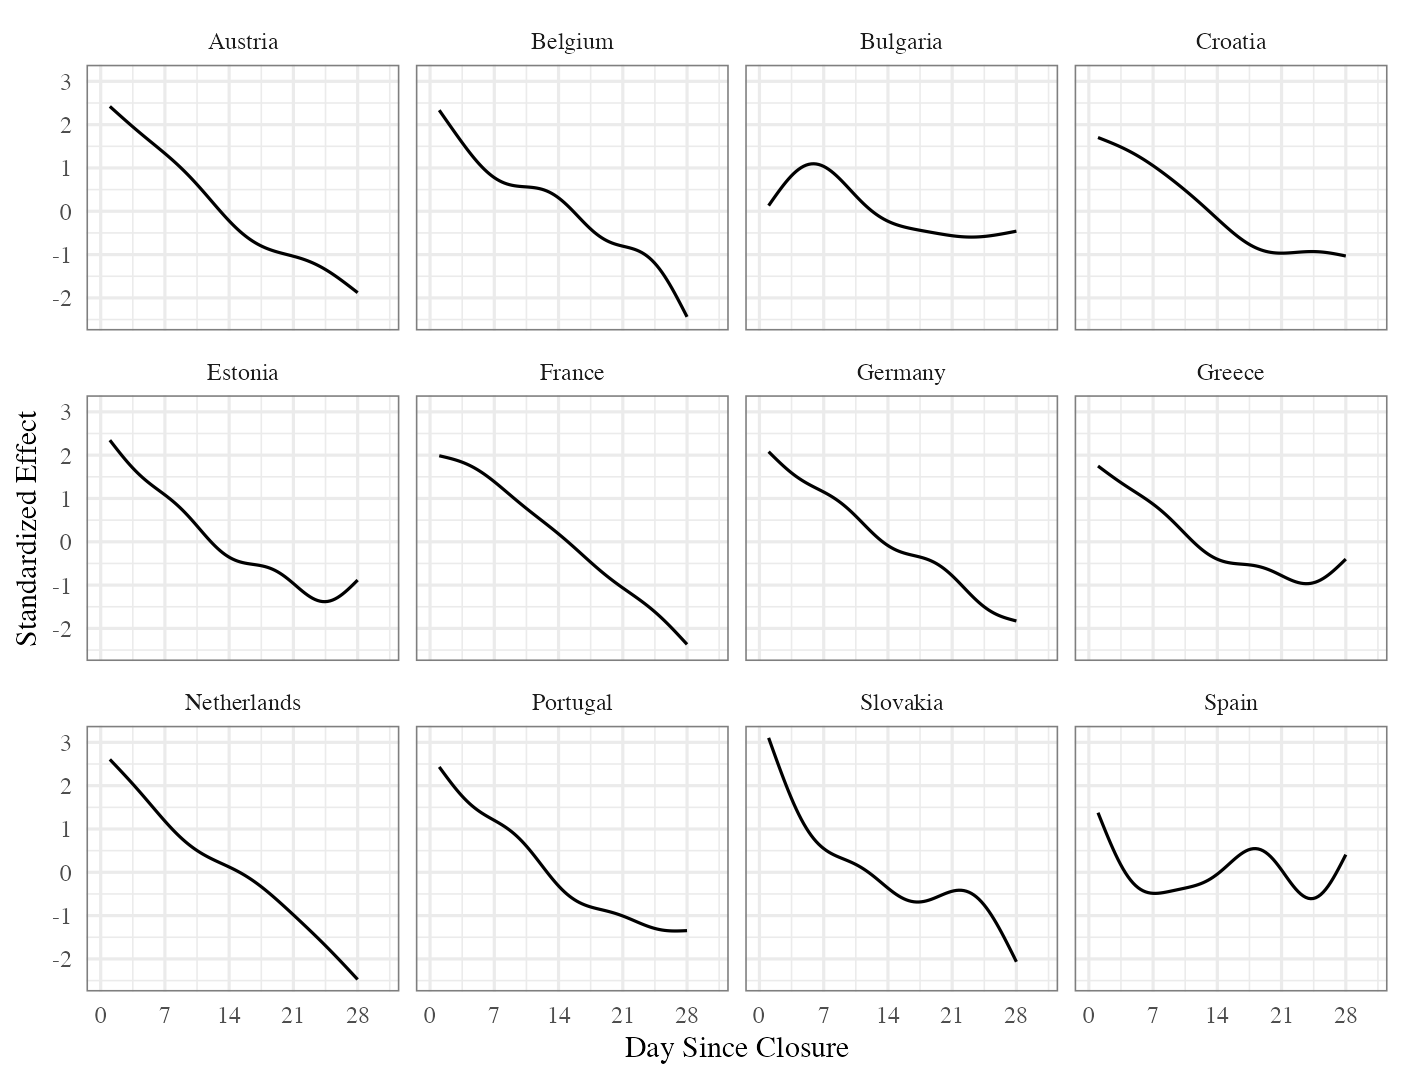
\includegraphics[width=\textwidth]{manuscript_files/figure-latex/country-1} \caption{Standardized effect of the smooth term in Generalized Additive Model by country.}\label{fig:country}
\end{figure}

\begin{figure}
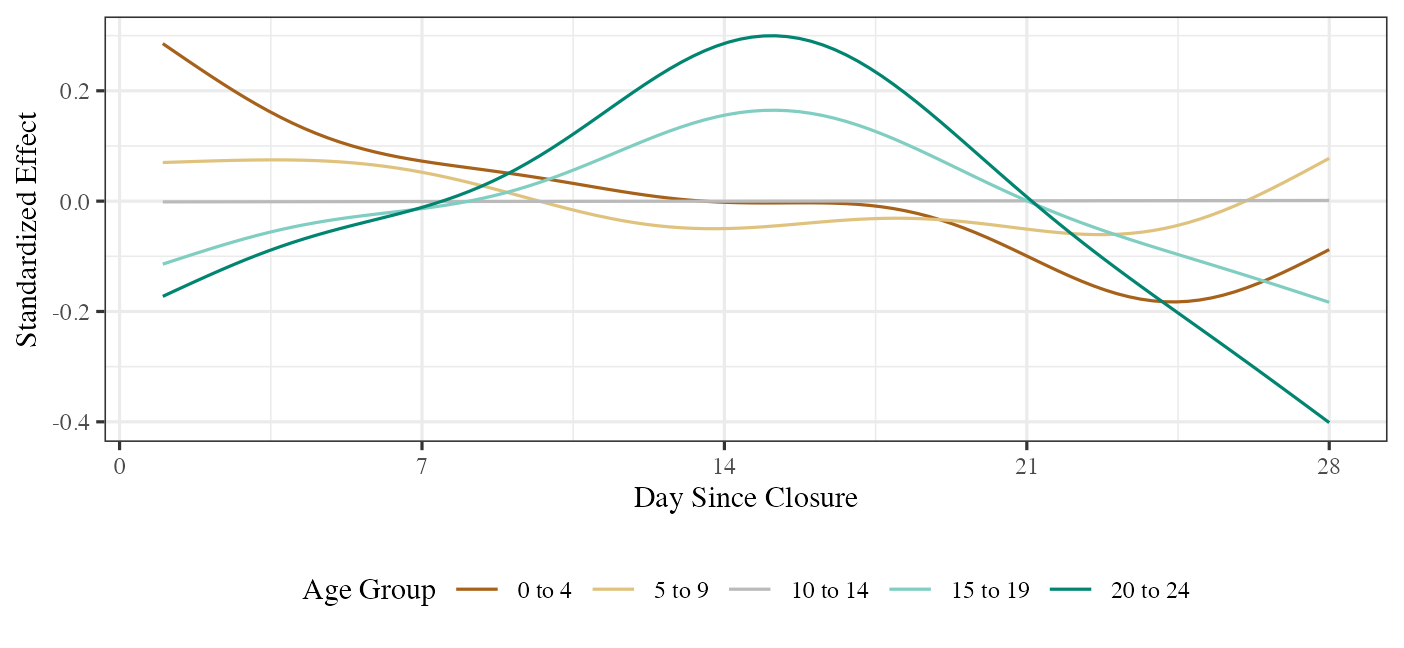
\includegraphics[width=\textwidth]{manuscript_files/figure-latex/age-1} \caption{Standardized effect of the smooth term in Generalized Additive Model by age group.}\label{fig:age}
\end{figure}

\begin{figure}[H]
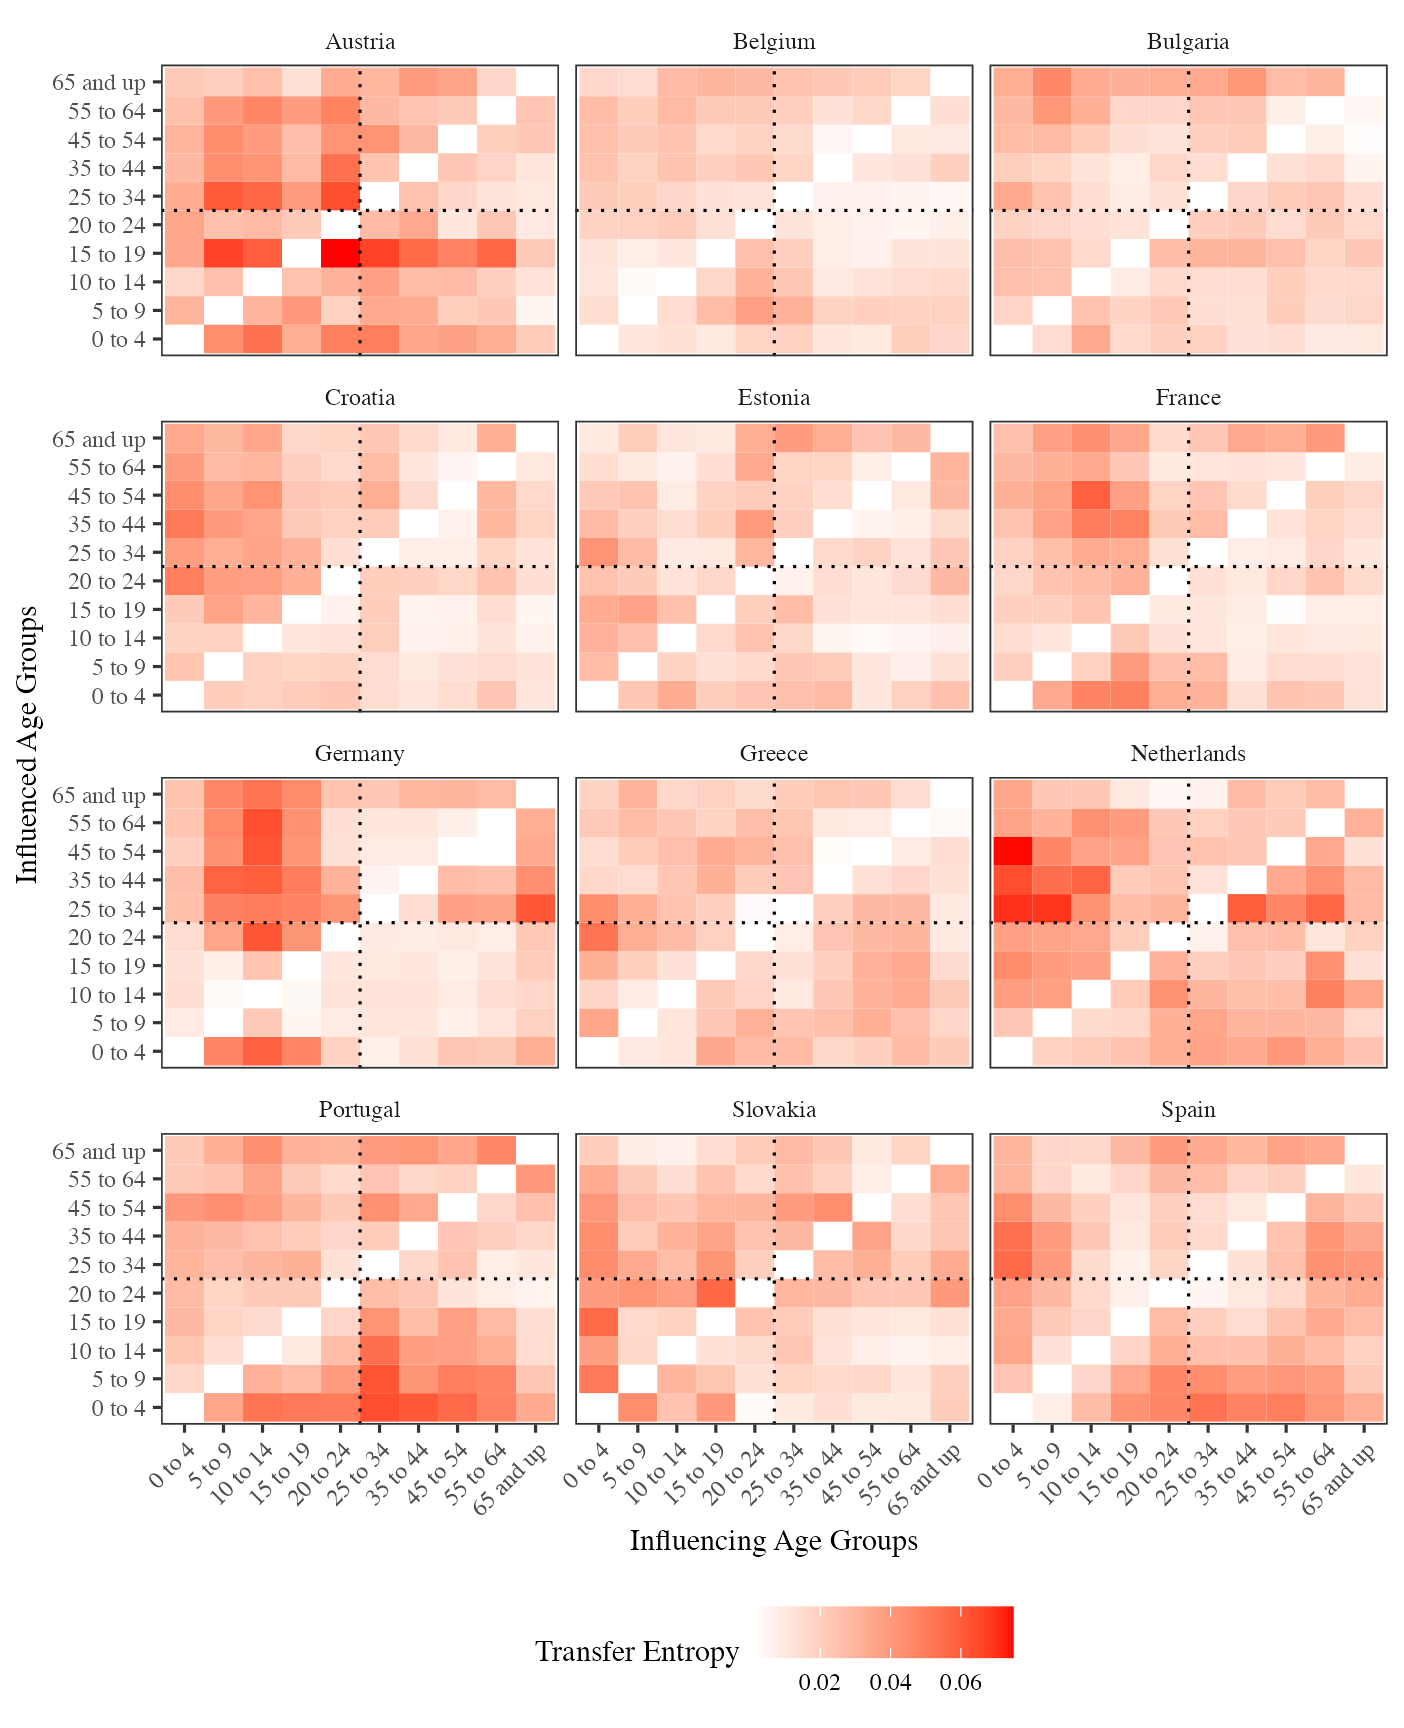
\includegraphics[width=\textwidth]{manuscript_files/figure-latex/te-1} \caption{Matrix of Transfer Entropy coefficients according to every age group combination for each of the selected European country. Age groups on the x-axis are influencing the age groups on the y-axis (\(ag\,x \rightarrow\,ag\,y\)). The significance of each Transfer Entropy coefficient is provided in Appendix 2.}\label{fig:te}
\end{figure}

Considering all countries, the analysis of age groups reveals distinct patterns (Figure \ref{fig:age}). For the 0 to 4 age group, i.e., the pre-school group, there was a downward trend during the initial two weeks following school closure, followed by flattening off (\(\chi^2(5.94) = 694.67\), \(p < 0.001\)). In contrast, for the age group ranging from 5 to 14, a substantial increase in cases after 14 days of school closure is found (5 to 9 age group: \(\chi^2(5.93) = 720.56\), \(p < 0.001\) and 10 to 14 age group: \(\chi^2(1) = 0.01\), \(p = 0.931\)). For age groups between 15 and 24, there is a notable surge immediately after school closure, followed by a decrease after 14 days (15 to 19 age group: \(\chi^2(4.97) = 8423.69\), \(p < 0.001\) and 20 to 24 age group: \(\chi^2(5.98) = 18932.54\), \(p < 0.001\)). Thus, while the total case number declined following school closures, among younger age groups only the pre-school age group had a consistent reduction in cases, while for other age groups, there was even an increase in cases following school closures.

Given that school closures were not only aimed at reducing COVID-19 cases among school-going children but also age groups, it is important to test the degree to which there was transmission across age groups, which is done using transfer entropy analysis. Before this analysis is carried out, an Augmented Dickey-Fuller has been applied to each age group to ensure that the daily changes in COVID-19 cases are stationary (see Appendix 1).

The results of the transfer entropy calculations between age groups for each of the 12 selected European countries are reported in Figure \ref{fig:te}. The absence of symmetry between influencing age groups (i.e., \(ag\,x\)) and influenced age groups (i.e., \(ag\,y\)) is found. Indeed, the change in COVID-19 cases in some age groups is influenced by other age groups, but they are not reciprocally influencing these age groups. Figure \ref{fig:te} shows how different age cohorts influence the COVID-19 case numbers of all age groups across countries. The upper left quadrant indicates how younger age cohorts are influencing older age cohorts, the bottom right quadrant indicates how older age cohorts are influencing younger age cohorts, finally, the lower left and upper right indicate how younger or older age cohorts are influencing themselves. By analyzing these quadrants, it is possible to identify similar patterns across multiple countries. Indeed, it appears that Austria, Germany, and The Netherlands have significantly higher \(T\) coefficients in the upper left quadrant of the matrix, which indicates that the daily changes in COVID-19 cases number in younger cohorts are predicting the daily changes in COVID-19 cases number in older cohorts. Alternatively, it appears that Austria, the Netherlands, Portugal, and Spain have significantly higher \(T\) coefficients in the lower right quadrant of the matrix, which indicates that the daily changes in COVID-19 cases number in older cohorts are predicting the daily changes in COVID-19 cases number in younger cohorts.

\hypertarget{discussion-conclusion}{%
\section{Discussion \& Conclusion}\label{discussion-conclusion}}

Knowledge about the transmission of the virus significantly improved over time as more studies have been published. While an early study found that children did not play an important role in the transmission of the virus (Li et al., 2020), more recent results give a more nuanced position, stating that the spread of the virus in children is moderate. This study, using robust statistical methods, considered the effect of school closures on COVID-19 cases across age groups. While there are commonalities in the evolution of COVID-19 cases across all European countries that were included in our data, school closures exhibit distinct impacts on different age groups. Notably, the analysis shows that the 0 to 4 age group experiences a downward trend in COVID-19 cases during the initial two weeks following school closure, followed by stabilization. In contrast, age groups ranging from 5 to 14 exhibit a substantial increase in cases after 14 days of school closure. Additionally, age groups between 15 and 24 demonstrate a notable surge immediately after school closure, followed by a decrease after 14 days. Thus, the results do not support the hypothesis that school closures were effective. These results partially replicate observations from Alfano (2022) while providing a clearer picture of the structure of the effect of school closure.

The Transfer Entropy calculations between age groups for each of the 12 selected European countries reveal an absence of symmetry between influencing age groups (X) and influenced age groups (Y). Some age groups influence the COVID-19 case numbers of other age groups, but there is no reciprocal influence. This finding suggests that changes in COVID-19 cases in certain age groups can predict the changes in other age groups but not vice versa, i.e., causality can be unidirectional. These findings highlight the importance of considering intergenerational interactions in designing effective control measures.

Furthermore, the quadrant analysis reveals similar patterns across multiple countries. Austria, Germany, and the Netherlands exhibit significantly higher TE coefficients in the upper left quadrant, indicating that changes in COVID-19 cases in younger cohorts predict the changes in older cohorts. On the other hand, Austria, the Netherlands, Portugal, and Spain show higher TE coefficients in the lower right quadrant, indicating that changes in COVID-19 cases in older cohorts predict the changes in younger cohorts.

In conclusion, this study sheds light on the trends and patterns of confirmed COVID-19 cases in selected European countries, with a particular focus on the influence of age groups and school closures. While a reduction in overall COVID-19 cases was found during school closures, which might suggest that like lockdowns (Alfano and Ercolano, 2020; Molefi et al., 2021), prolonged school closures could contribute to mitigating the spread of the virus, the results for the school-going age groups suggest that this is not the case.

\hypertarget{data-availability}{%
\section{Data Availability}\label{data-availability}}

All data extracted from the COVerAGE-DB project and from the UNESCO global education coalition that are used to produce these results are fully available here \url{https://github.com/damien-dupre/covid_ts_causality}. The repository also includes the R code that were used to produce these results.

\hypertarget{references}{%
\section*{References}\label{references}}
\addcontentsline{toc}{section}{References}

\hypertarget{refs}{}
\begin{CSLReferences}{1}{0}
\leavevmode\vadjust pre{\hypertarget{ref-alfano2022effects}{}}%
Alfano, V., 2022. The effects of school closures on COVID-19: A cross-country panel analysis. Applied Health Economics and Health Policy 20, 223--233. doi:\href{https://doi.org/10.1007/s40258-021-00702-z}{10.1007/s40258-021-00702-z}

\leavevmode\vadjust pre{\hypertarget{ref-alfano2020efficacy}{}}%
Alfano, V., Ercolano, S., 2020. The efficacy of lockdown against COVID-19: A cross-country panel analysis. Applied Health Economics and Health Policy 18, 509--517. doi:\href{https://doi.org/10.1007/s40258-020-00596-3}{10.1007/s40258-020-00596-3}

\leavevmode\vadjust pre{\hypertarget{ref-ard2023lauterbach}{}}%
ARD tagesschau, 2023.

\leavevmode\vadjust pre{\hypertarget{ref-barnett2009granger}{}}%
Barnett, L., Barrett, A.B., Seth, A.K., 2009. Granger causality and transfer entropy are equivalent for gaussian variables. Physical Review Letters 103, 2387011--2387014. doi:\href{https://doi.org/10.1103/PhysRevLett.103.238701}{10.1103/PhysRevLett.103.238701}

\leavevmode\vadjust pre{\hypertarget{ref-bayham2020impact}{}}%
Bayham, J., Fenichel, E.P., 2020. Impact of school closures for COVID-19 on the US health-care workforce and net mortality: A modelling study. The Lancet Public Health 5, e271--e278. doi:\href{https://doi.org/10.1016/S2468-2667(20)30082-7}{10.1016/S2468-2667(20)30082-7}

\leavevmode\vadjust pre{\hypertarget{ref-behrendt2019rtransferentropy}{}}%
Behrendt, S., Dimpfl, T., Peter, F.J., Zimmermann, D.J., 2019. RTransferEntropy --- quantifying information flow between different time series using effective transfer entropy. SoftwareX 10. doi:\href{https://doi.org/10.1016/j.softx.2019.100265}{10.1016/j.softx.2019.100265}

\leavevmode\vadjust pre{\hypertarget{ref-chang2020modelling}{}}%
Chang, S.L., Harding, N., Zachreson, C., Cliff, O.M., Prokopenko, M., 2020. Modelling transmission and control of the COVID-19 pandemic in australia. Nature Communications 11, 1--13. doi:\href{https://doi.org/10.1038/s41467-020-19393-6}{10.1038/s41467-020-19393-6}

\leavevmode\vadjust pre{\hypertarget{ref-de2021determines}{}}%
De Simone, E., Mourao, P.R., 2021. What determines governments' response time to COVID-19? A cross-country inquiry on the measure restricting internal movements. Open Economics 4, 106--117. doi:\href{https://doi.org/10.1515/openec-2020-0116}{10.1515/openec-2020-0116}

\leavevmode\vadjust pre{\hypertarget{ref-esposito2021comprehensive}{}}%
Esposito, S., Cotugno, N., Principi, N., 2021. Comprehensive and safe school strategy during COVID-19 pandemic. Italian Journal of Pediatrics 47, 1--4. doi:\href{https://doi.org/10.1186/s13052-021-00960-6}{10.1186/s13052-021-00960-6}

\leavevmode\vadjust pre{\hypertarget{ref-fukumoto2021no}{}}%
Fukumoto, K., McClean, C.T., Nakagawa, K., 2021. No causal effect of school closures in japan on the spread of COVID-19 in spring 2020. Nature Medicine 27, 2111--2119. doi:\href{https://doi.org/10.1038/s41591-021-01571-8}{10.1038/s41591-021-01571-8}

\leavevmode\vadjust pre{\hypertarget{ref-grasleguen2021reopening}{}}%
Gras-Le Guen, C., Cohen, R., Rozenberg, J., Launay, E., Levy-Bruhl, D., Delacourt, C., 2021. Reopening schools in the context of increasing COVID-19 community transmission: The french experience. Archives de Pédiatrie 28, 178--185. doi:\href{https://doi.org/10.1016/j.arcped.2021.02.001}{10.1016/j.arcped.2021.02.001}

\leavevmode\vadjust pre{\hypertarget{ref-heavey2020evidence}{}}%
Heavey, L., Casey, G., Kelly, C., Kelly, D., McDarby, G., 2020. No evidence of secondary transmission of COVID-19 from children attending school in ireland, 2020. Eurosurveillance 25, 1--4. doi:\href{https://doi.org/10.2807/1560-7917.ES.2020.25.21.2000903}{10.2807/1560-7917.ES.2020.25.21.2000903}

\leavevmode\vadjust pre{\hypertarget{ref-vanderhoek2020role}{}}%
Hoek, W. van der, Backer, J.A., Bodewes, R., Friesema, I., Meijer, A., Pijnacker, R., Reukers, D.F.M., Reusken, C., Roof, I., Rots, N., Te Wierik, M.J.M., Gageldonk-Lafeber, A. van, Waegemaekers, C., Hof, S. van den, 2020. \href{https://www.ntvg.nl/artikelen/de-rol-van-kinderen-de-transmissie-van-sars-cov-2}{De rol van kinderen in de transmissie van SARS-CoV-2}. Nederlands Tijdschrift voor Geneeskunde 164, 1--7.

\leavevmode\vadjust pre{\hypertarget{ref-iwata2020school}{}}%
Iwata, K., Doi, A., Miyakoshi, C., 2020. Was school closure effective in mitigating coronavirus disease 2019 (COVID-19)? Time series analysis using bayesian inference. International Journal of Infectious Diseases 99, 57--61. doi:\href{https://doi.org/10.1016/j.ijid.2020.07.052}{10.1016/j.ijid.2020.07.052}

\leavevmode\vadjust pre{\hypertarget{ref-kawano2015substantial}{}}%
Kawano, S., Kakehashi, M., 2015. Substantial impact of school closure on the transmission dynamics during the pandemic flu H1N1-2009 in oita, japan. PloS one 10, e0144839. doi:\href{https://doi.org/10.1371/journal.pone.0144839}{10.1371/journal.pone.0144839}

\leavevmode\vadjust pre{\hypertarget{ref-kim2021role}{}}%
Kim, J., Choe, Y.J., Lee, J., Park, Y.J., Park, O., Han, M.S., Kim, J.-H., Choi, E.H., 2021. Role of children in household transmission of COVID-19. Archives of Disease in Childhood 106, 709--711. doi:\href{https://doi.org/10.1136/archdischild-2020-319910}{10.1136/archdischild-2020-319910}

\leavevmode\vadjust pre{\hypertarget{ref-kissler2020symbolic}{}}%
Kissler, S.M., Viboud, C., Grenfell, B.T., Gog, J.R., 2020. Symbolic transfer entropy reveals the age structure of pandemic influenza transmission from high-volume influenza-like illness data. Journal of the Royal Society Interface 17, 1--9. doi:\href{https://doi.org/10.1098/rsif.2019.0628}{10.1098/rsif.2019.0628}

\leavevmode\vadjust pre{\hypertarget{ref-lerkkanen2023reading}{}}%
Lerkkanen, M.-K., Pakarinen, E., Salminen, J., Torppa, M., 2023. Reading and math skills development among finnish primary school children before and after COVID-19 school closure. Reading and Writing 36, 263--288. doi:\href{https://doi.org/10.1007/s11145-022-10358-3}{10.1007/s11145-022-10358-3}

\leavevmode\vadjust pre{\hypertarget{ref-li2020role}{}}%
Li, X., Xu, W., Dozier, M., He, Y., Kirolos, A., Theodoratou, E., others, 2020. The role of children in transmission of SARS-CoV-2: A rapid review. Journal of Global Health 10, 1--10. doi:\href{https://doi.org/10.7189/jogh.10.011101}{10.7189/jogh.10.011101}

\leavevmode\vadjust pre{\hypertarget{ref-loader2006local}{}}%
Loader, C., 2006. Local regression and likelihood. Springer, New York, NY.

\leavevmode\vadjust pre{\hypertarget{ref-ludvigsson2020children}{}}%
Ludvigsson, J.F., 2020. Children are unlikely to be the main drivers of the COVID-19 pandemic -- a systematic review. Acta Paediatrica 109, 1525--1530. doi:\href{https://doi.org/10.1111/apa.15371}{10.1111/apa.15371}

\leavevmode\vadjust pre{\hypertarget{ref-molefi2021impact}{}}%
Molefi, M., Tlhakanelo, J.T., Phologolo, T., Hamda, S.G., Masupe, T., Tsima, B., Setlhare, V., Mashalla, Y., Wiebe, D.J., others, 2021. The impact of china's lockdown policy on the incidence of CoVID-19: An interrupted time series analysis. BioMed Research International 2021. doi:\href{https://doi.org/10.1155/2021/9498029}{10.1155/2021/9498029}

\leavevmode\vadjust pre{\hypertarget{ref-moser2018estimating}{}}%
Moser, C.B., White, L.F., 2018. Estimating age-specific reproductive numbers---a comparison of methods. Statistical Methods in Medical Research 27, 2050--2059. doi:\href{https://doi.org/10.1177/0962280216673676}{10.1177/0962280216673676}

\leavevmode\vadjust pre{\hypertarget{ref-moulin2022longitudinal}{}}%
Moulin, F., Bailhache, M., Monnier, M., Thierry, X., Vandentorren, S., Côté, S.M., Falissard, B., Simeon, T., Geay, B., Marchand, L., others, 2022. Longitudinal impact of psychosocial status on children's mental health in the context of COVID-19 pandemic restrictions. European Child \& Adolescent Psychiatry 1--10. doi:\href{https://doi.org/10.1007/s00787-022-02010-w}{10.1007/s00787-022-02010-w}

\leavevmode\vadjust pre{\hypertarget{ref-riffe2021data}{}}%
Riffe, T., Acosta, E., COVerAGE-DB team, the, 2021. {Data Resource Profile: COVerAGE-DB: a global demographic database of COVID-19 cases and deaths}. International Journal of Epidemiology 50, 390--390f. doi:\href{https://doi.org/10.1093/ije/dyab027}{10.1093/ije/dyab027}

\leavevmode\vadjust pre{\hypertarget{ref-schreiber2000measuring}{}}%
Schreiber, T., 2000. Measuring information transfer. Physical Review Letters 85, 461--464. doi:\href{https://doi.org/10.1103/PhysRevLett.85.461}{10.1103/PhysRevLett.85.461}

\leavevmode\vadjust pre{\hypertarget{ref-shannon1948mathematical}{}}%
Shannon, C.E., 1948. A mathematical theory of communication. The Bell System Technical Journal 27, 379--423. doi:\href{https://doi.org/10.1002/j.1538-7305.1948.tb01338.x}{10.1002/j.1538-7305.1948.tb01338.x}

\leavevmode\vadjust pre{\hypertarget{ref-siebach2021childhood}{}}%
Siebach, M.K., Piedimonte, G., Ley, S.H., 2021. COVID-19 in childhood: Transmission, clinical presentation, complications and risk factors. Pediatric Pulmonology 56, 1342--1356. doi:\href{https://doi.org/10.1002/ppul.25344}{10.1002/ppul.25344}

\leavevmode\vadjust pre{\hypertarget{ref-sorianoarandes2021household}{}}%
Soriano-Arandes, A., Gatell, A., Serrano, P., Biosca, M., Campillo, F., Capdevila, R., Fàbrega, A., Lobato, Z., López, N., Moreno, A.M., Poblet, M., Riera-Bosch, M.T., Rius, N., Ruiz, M., Sánchez, A., Valldepérez, C., Vilà, M., Pineda, V., Lazcano, U., Díaz, Y., Reyes-Urueña, J., Soler-Palacín, P., Catalonia Research Group, C.P.D. in, 2021. Household severe acute respiratory syndrome coronavirus 2 transmission and children: A network prospective study. Clinical Infectious Diseases 73, e1261--e1269. doi:\href{https://doi.org/10.1093/cid/ciab228}{10.1093/cid/ciab228}

\leavevmode\vadjust pre{\hypertarget{ref-stage2021shut}{}}%
Stage, H.B., Shingleton, J., Ghosh, S., Scarabel, F., Pellis, L., Finnie, T., 2021. Shut and re-open: The role of schools in the spread of COVID-19 in europe. Philosophical Transactions of the Royal Society B 376, 1--11. doi:\href{https://doi.org/10.1098/rstb.2020.0277}{10.1098/rstb.2020.0277}

\leavevmode\vadjust pre{\hypertarget{ref-sugimoto2023temporal}{}}%
Sugimoto, M., Murakami, K., Sasaki, S., 2023. Temporal patterns of sleep and eating among children during school closure in japan due to COVID-19 pandemic: Associations with lifestyle behaviours and dietary intake. Public Health Nutrition 26, 393--407. doi:\href{https://doi.org/10.1017/S1368980022001148}{10.1017/S1368980022001148}

\leavevmode\vadjust pre{\hypertarget{ref-yoshiyuki2020effects}{}}%
Sugishita, J.A.S., Yoshiyuki AND Kurita, 2020. Effects of voluntary event cancellation and school closure as countermeasures against COVID-19 outbreak in japan. PLOS ONE 15, 1--10. doi:\href{https://doi.org/10.1371/journal.pone.0239455}{10.1371/journal.pone.0239455}

\leavevmode\vadjust pre{\hypertarget{ref-unesco2022https}{}}%
{UNESCO} global education coalition, 2022.

\leavevmode\vadjust pre{\hypertarget{ref-walsh2021school}{}}%
Walsh, S., Chowdhury, A., Braithwaite, V., Russell, S., Birch, J.M., Ward, J.L., Waddington, C., Brayne, C., Bonell, C., Viner, R.M., others, 2021. Do school closures and school reopenings affect community transmission of COVID-19? A systematic review of observational studies. BMJ Open 11, e053371. doi:\href{https://doi.org/10.1136/bmjopen-2021-053371}{10.1136/bmjopen-2021-053371}

\leavevmode\vadjust pre{\hypertarget{ref-wood2011fast}{}}%
Wood, S.N., 2011. Fast stable restricted maximum likelihood and marginal likelihood estimation of semiparametric generalized linear models. Journal of the Royal Statistical Society (B) 73, 3--36. doi:\href{https://doi.org/10.1111/j.1467-9868.2010.00749.x}{10.1111/j.1467-9868.2010.00749.x}

\leavevmode\vadjust pre{\hypertarget{ref-wood2017generalized}{}}%
Wood, S.N., 2017. Generalized additive models: An introduction with r. CRC, Boca Raton, FL.

\leavevmode\vadjust pre{\hypertarget{ref-who2022https}{}}%
World health organization COVID-19 data, 2022.

\leavevmode\vadjust pre{\hypertarget{ref-zhendong2020clinical}{}}%
Zhen-Dong, Y., Gao-Jun, Z., Run-Ming, J., Zhi-Sheng, L., Zong-Qi, D., Xiong, X., Guo-Wei, S., 2020. Clinical and transmission dynamics characteristics of 406 children with coronavirus disease 2019 in china: A review. Journal of Infection 81, e11--e15. doi:\href{https://doi.org/10.1016/j.jinf.2020.04.030}{10.1016/j.jinf.2020.04.030}

\end{CSLReferences}

\end{document}
